\documentclass[letterpaper,11pt]{article}
\usepackage{graphicx}
\usepackage{listings}
\usepackage[super]{nth}
\usepackage[hyphens]{url}
\usepackage{hyperref}
\usepackage{amsmath}
\usepackage[makeroom]{cancel}
\usepackage[table]{xcolor}
\usepackage{comment}
\usepackage[space]{grffile}
\usepackage{csvsimple}

\newcommand*{\srcPath}{../src}%

\lstset{
	basicstyle=\footnotesize,
	breaklines=true,
}

\begin{document}

\begin{titlepage}

\begin{center}

\Huge{Assignment 6}

\Large{CS 532:  Introduction to Web Science}

\Large{Spring 2017}

\Large{Grant Atkins}

\Large Finished on \today

\end{center}

\end{titlepage}

\newpage


% =================================
% First question
% =================================
\section*{1}

\subsection*{Question}

\begin{verbatim}
1.  D3 graphing (10 points)

Use D3 to visualize your Twitter followers.  Use my twitter account
("@phonedude_mln") if you do not have >= 50 followers.  For example,
@hvdsomp follows me, as does @mart1nkle1n.  They also follow each
other, so they would both have links to me and links to each other.

To see if two users follow each other, see:
https://dev.twitter.com/rest/reference/get/friendships/show

Attractiveness of the graph counts!  Nodes should be labeled (avatar
images are even better), and edge types (follows, following) should
be marked.

Note: for getting GitHub to serve HTML (and other media types), see:
http://stackoverflow.com/questions/6551446/
can-i-run-html-files-directly-from-github-instead-of-just-viewing-their-source

Be sure to include the URI(s) for your D3 graph in your report. 
\end{verbatim}

\clearpage
\subsection*{Answer}



% \begin{figure}[h]
% \centering
% 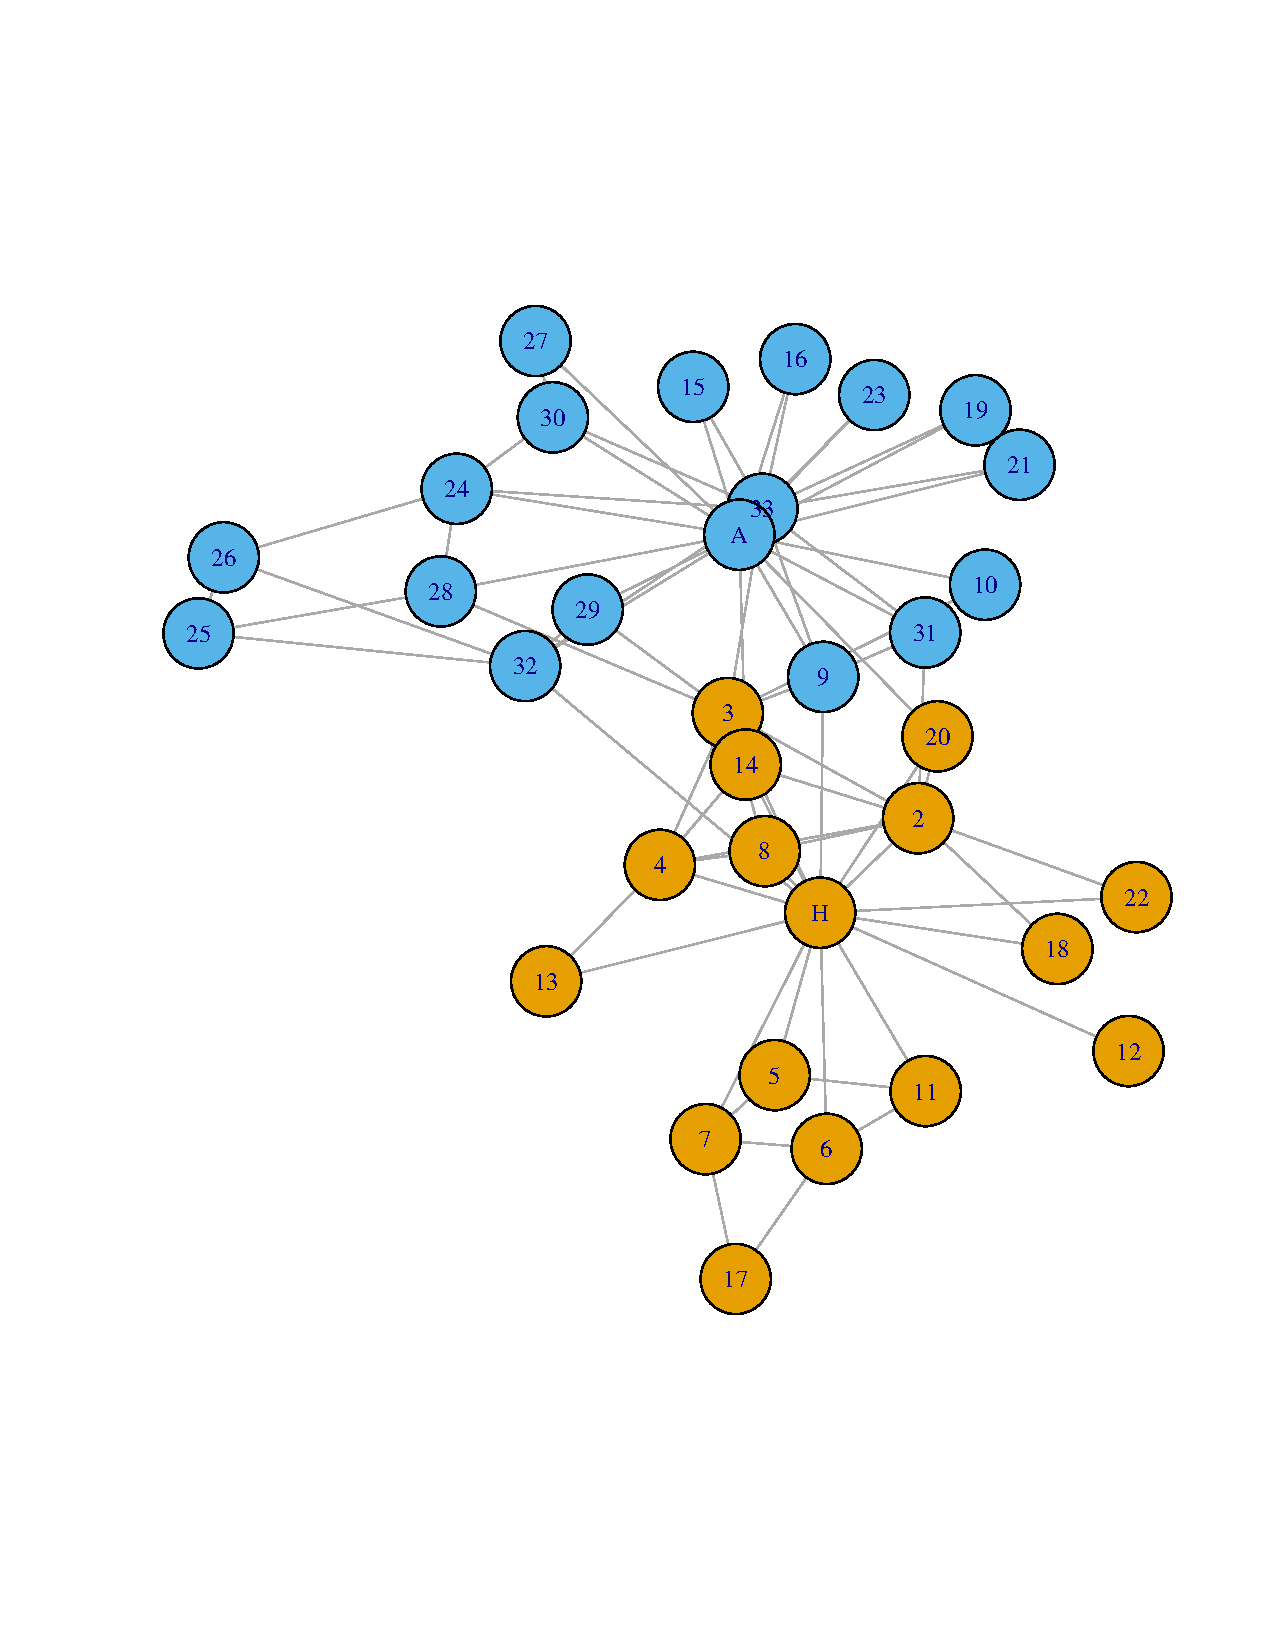
\includegraphics[scale=0.6]{originalSplit.pdf}
% \caption{Original Karate Club Split}
% \label{fig:q1orig}
% \end{figure}

% \lstinputlisting[frame=single,caption={R script for splitting groups using Girvan-Newman algorithm},label=lst:rscript,captionpos=b,numbers=left,showspaces=false,showstringspaces=false,basicstyle=\footnotesize]{\srcPath/karateClub.R}



\clearpage

% =================================
% Second question
% =================================

\section*{2}

\subsection*{Question}

\begin{verbatim}
Extra credit: (5 points)

2.  Gender homophily in your Twitter graph 

Take the Twitter graph you generated in question #1 and test for
male-female homophily.  For the purposes of this question you can
consider the graph as undirected (i.e., no distinction between
"follows" and "following").  Use the twitter name (not "screen
name"; for example "Michael L. Nelson" and not "@phonedude_mln")
and programatically determine if the user is male or female.  Some
sites that might be useful:

https://genderize.io/
https://pypi.python.org/pypi/gender-detector/0.0.4

Create a table of Twitter users and their likely gender.  List any 
accounts that can't be determined and remove them from the graph.

Perform the homophily test as described in slides 11-16, Week 8.

Does your Twitter graph exhibit gender homophily?
\end{verbatim}

\clearpage
\subsection*{Answer}

% \begin{figure}[h]
% \centering
% 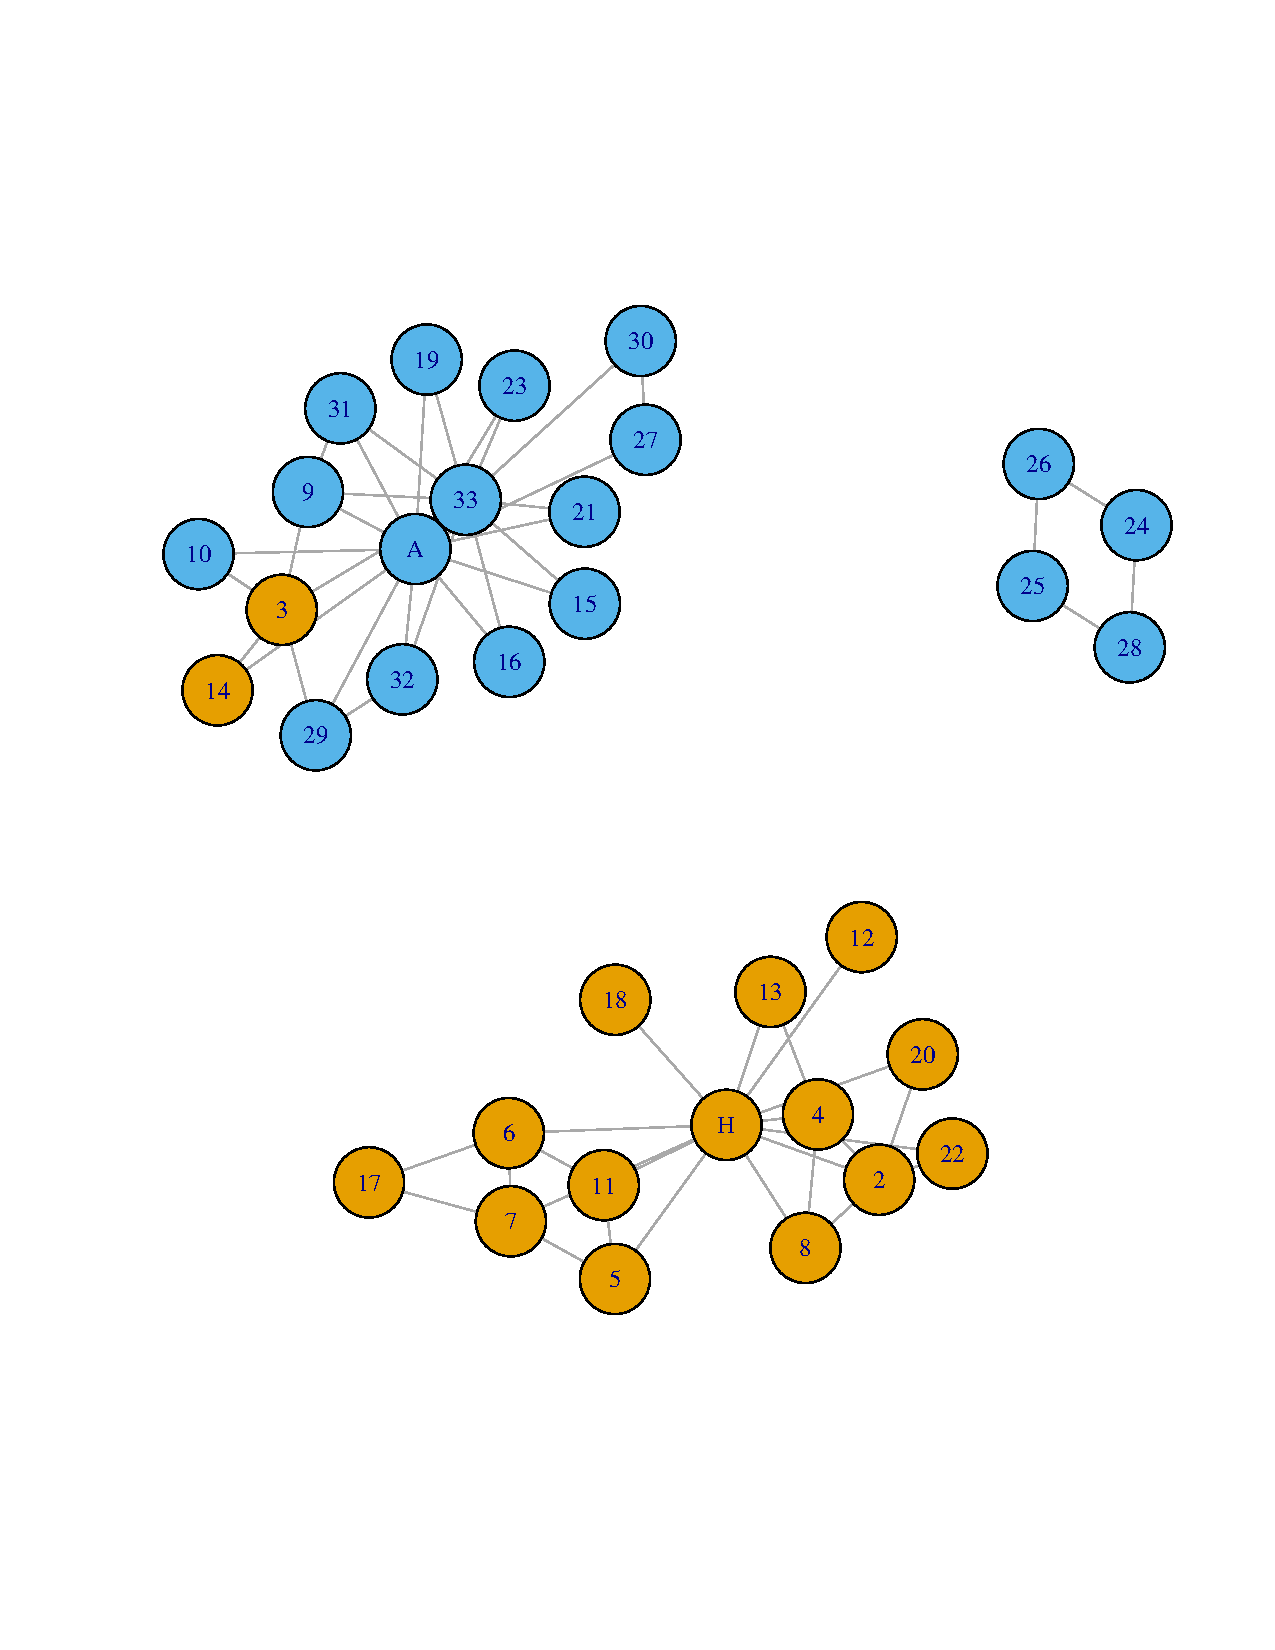
\includegraphics[scale=0.6]{predictedSplit3.pdf}
% \caption{Group split of 3 with Girvan-Newman algorithm from karateClub.R}
% \label{fig:split3}
% \end{figure}

\clearpage

% =================================
% 3rd question
% =================================

\section*{3}

\subsection*{Question}

\begin{verbatim}
Extra credit: (3 points)

3.  Using D3, create a graph of the Karate club before and after
the split.

- Weight the edges with the data from: 
http://vlado.fmf.uni-lj.si/pub/networks/data/ucinet/zachary.dat

- Have the transition from before/after the split occur on a mouse
click.  This is a toggle, so the graph will go back and forth beween
connected and disconnected.
\end{verbatim}

\clearpage
\subsection*{Answer}

% \begin{figure}[h]
% \centering
% 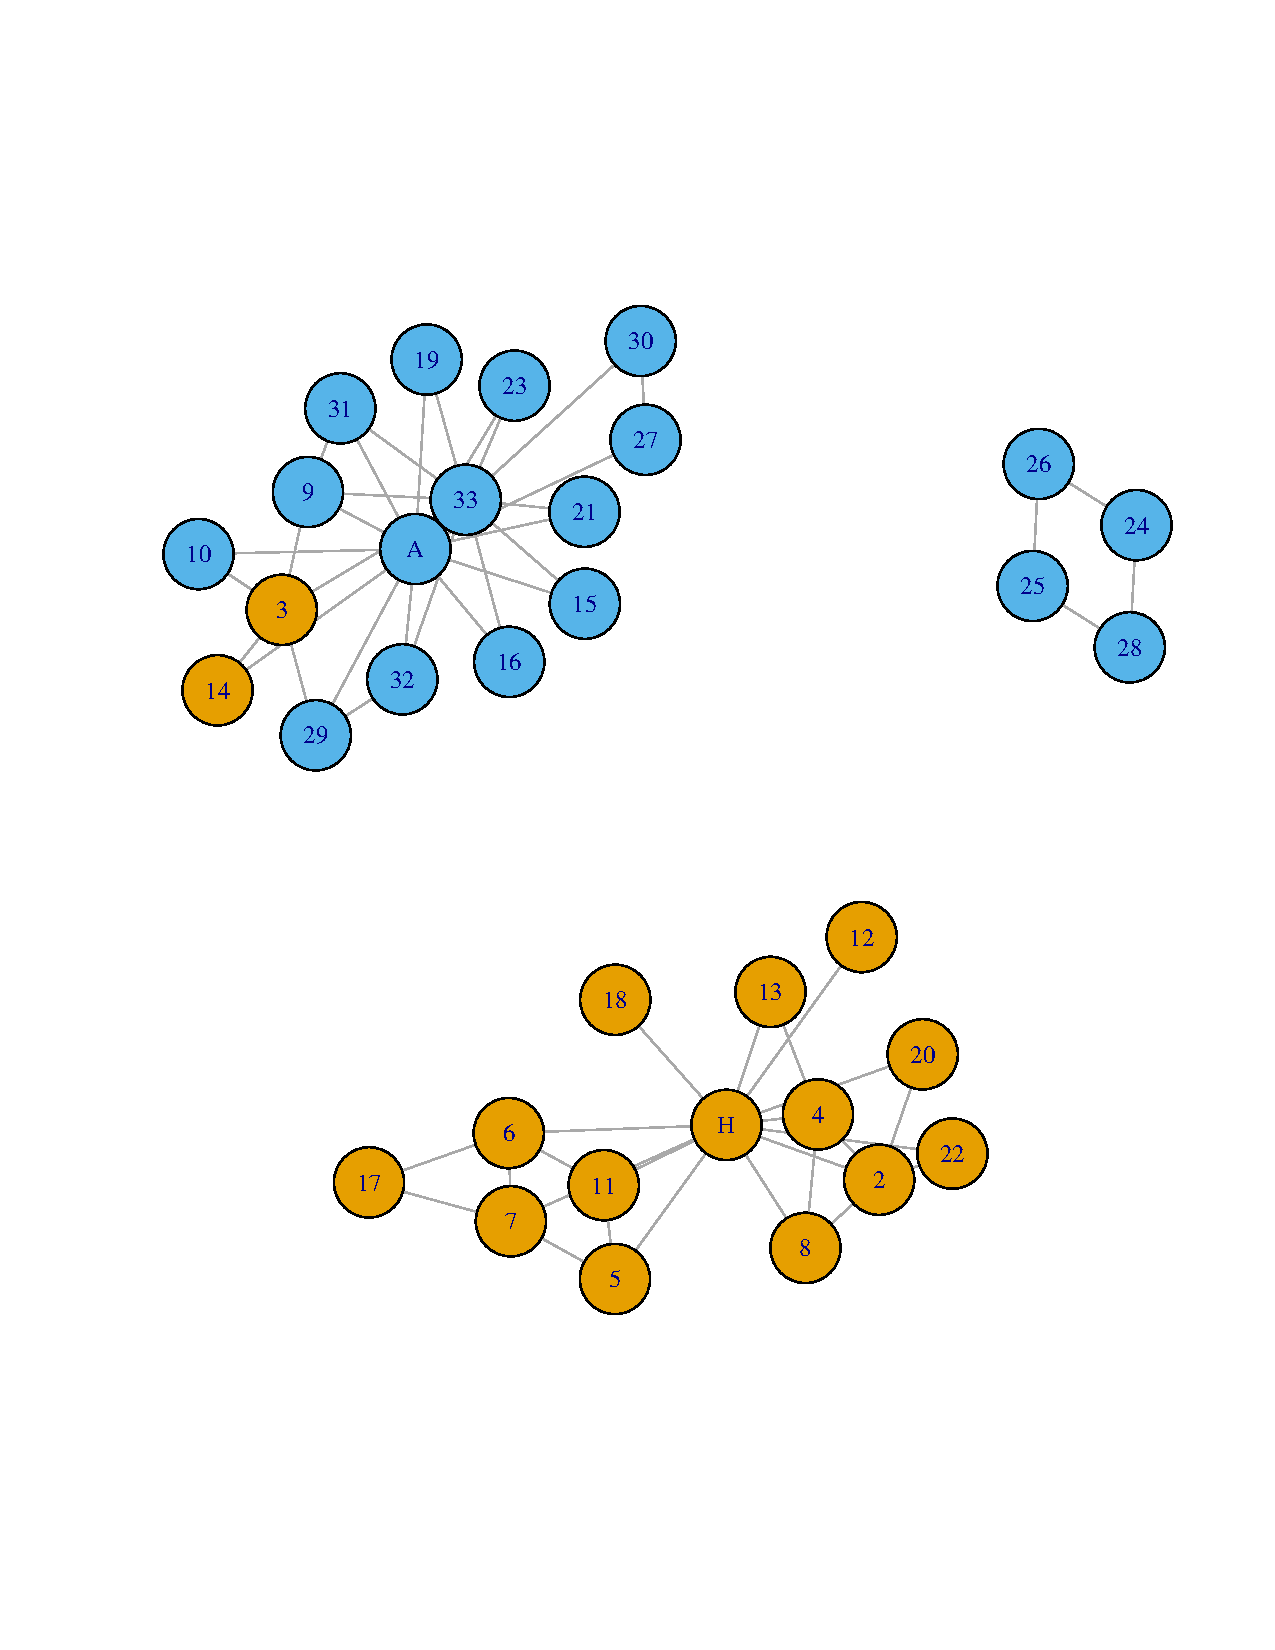
\includegraphics[scale=0.6]{predictedSplit3.pdf}
% \caption{Group split of 3 with Girvan-Newman algorithm from karateClub.R}
% \label{fig:split3}
% \end{figure}

\clearpage

% =================================
% Bibliography
% =================================

\begin{thebibliography}{9}
\bibitem{igraphdataref}
Csardi, Gabor. ``Package `graphdata' '' iGraphData. Cran-R-Project, 13 July 2015. Web. 16 March 2017.\url{https://cran.r-project.org/web/packages/igraphdata/igraphdata.pdf}.
\bibitem{igraphref}
Csardi, Gabor, ``Package `igraph' '' iGraph. Cran-R-Project, 13 July 2015. Web. 16 March 2017. \url{http://igraph.org/r/doc/igraph.pdf}.
\bibitem{commref}
Rodrigues, David.``Finding Communities in networks with R and igraph'' N.p., n.d. Web. 16 March 2017. \url{http://www.sixhat.net/finding-communities-in-networks-with-r-and-igraph.html}.
\bibitem{zachref}
W. W. Zachary, An information flow model for conflict and fission in small groups, Journal of Anthropological Research 33, 452-473 (1977).
\end{thebibliography}

\end{document}